\section{Discussion}

\subsection{Max Speed}
\begin{figure}[!htb]

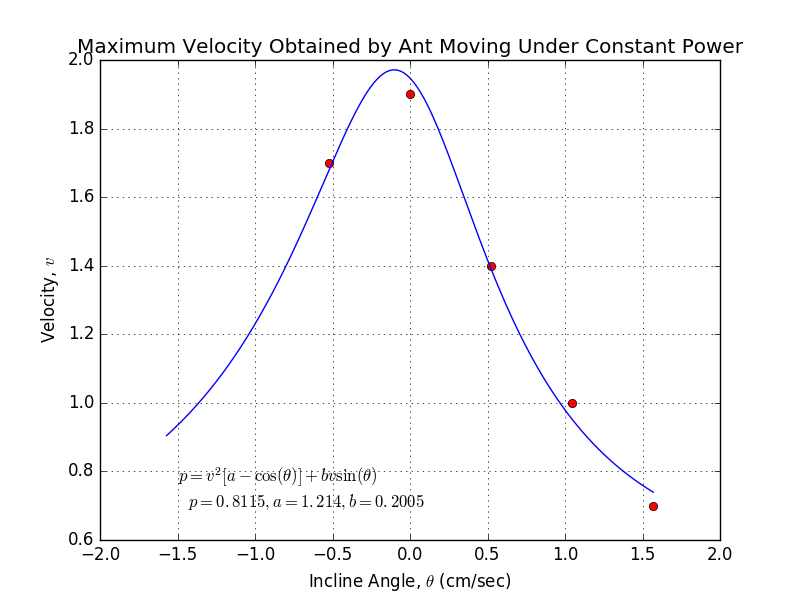
\includegraphics[width=0.4\textwidth]{img/const_power_velocity}

\end{figure}
\begin{align*}
 p = v^2(a - \cos(\theta)) + b \times v \times \sin(\theta) \\
  a = 1.214 \\
  b = 0.2005 \\
  p = 0.8115
\end{align*}


\subsection{Optimal Corner-to-Corner}
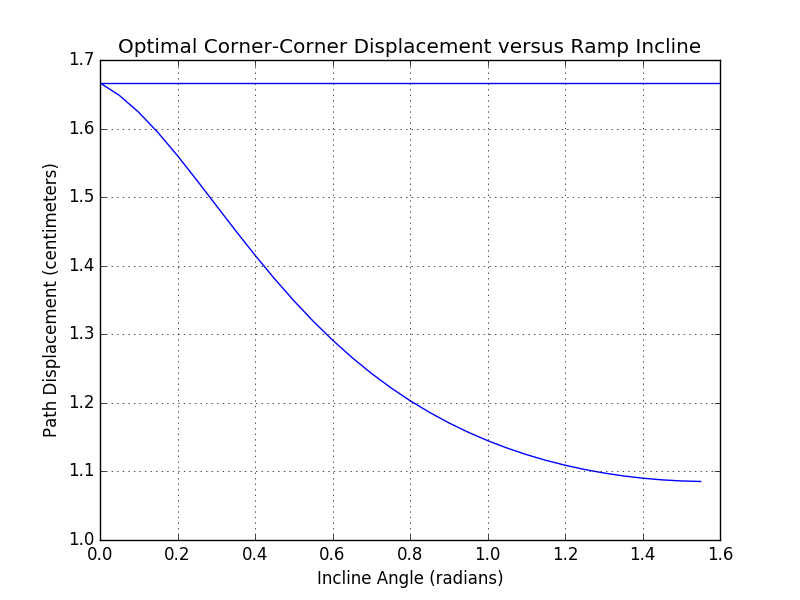
\includegraphics[width=0.5\textwidth]{img/optimal_corner_corner_displacement_versus_ramp_incline}
\begin{center}
\begin{tabular}{ c c c }
 incline & displacement (cm) & time (sec) \\ 
 0 & 1.6666666951743492 & 16.239124992741537 \\  
 math.pi/6 & 1.3347182872155725 & 18.030748007672663 \\
 math.pi/4 & 1.2086175733441706 & 18.955404943299744 \\
 math.pi/3 & 1.1347489653055225 & 19.589063308764256 \\
 math.pi/2 & 1.0852990219701015 & 20.06002493694109
\end{tabular} \\
\end{center}
displacement for a direct path: 1.666666666666667 cm

\subsection{Optimal Center-to-Center Path}
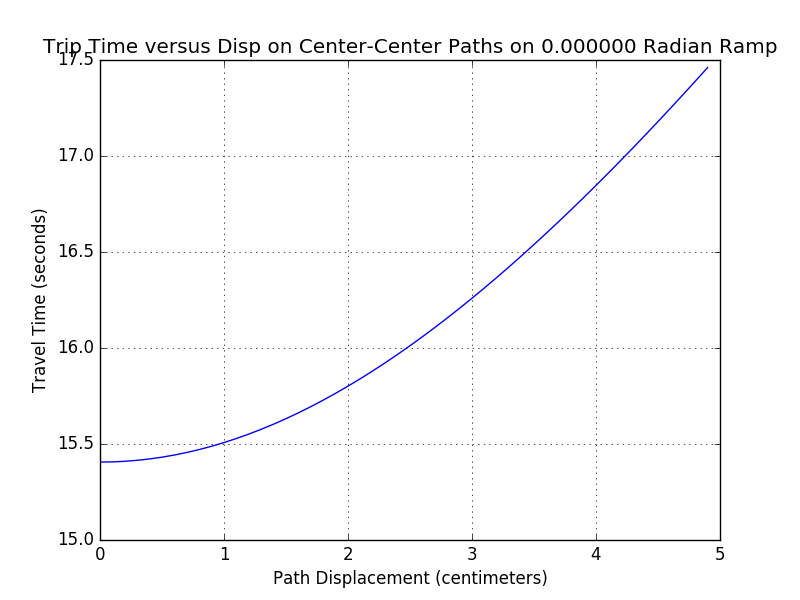
\includegraphics[width=0.2\textwidth]{img/center_center_trip_time_vs_displacement_0_radian_ramp}%
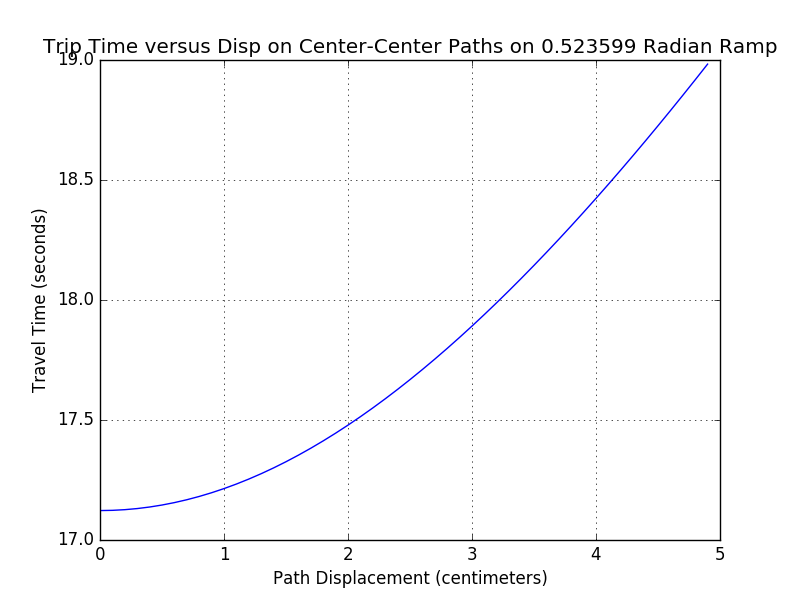
\includegraphics[width=0.2\textwidth]{img/center_center_trip_time_vs_displacement_pi_6_radian_ramp}%
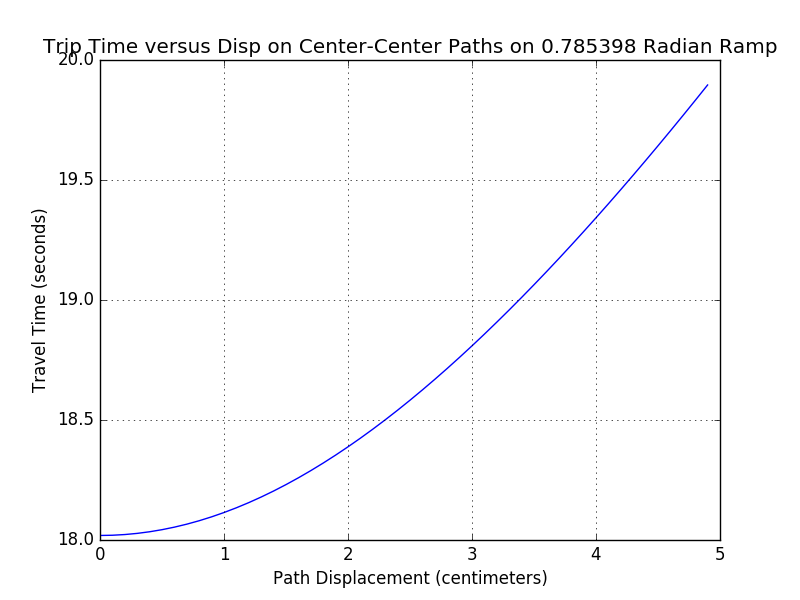
\includegraphics[width=0.2\textwidth]{img/center_center_trip_time_vs_displacement_pi_4_radian_ramp}%
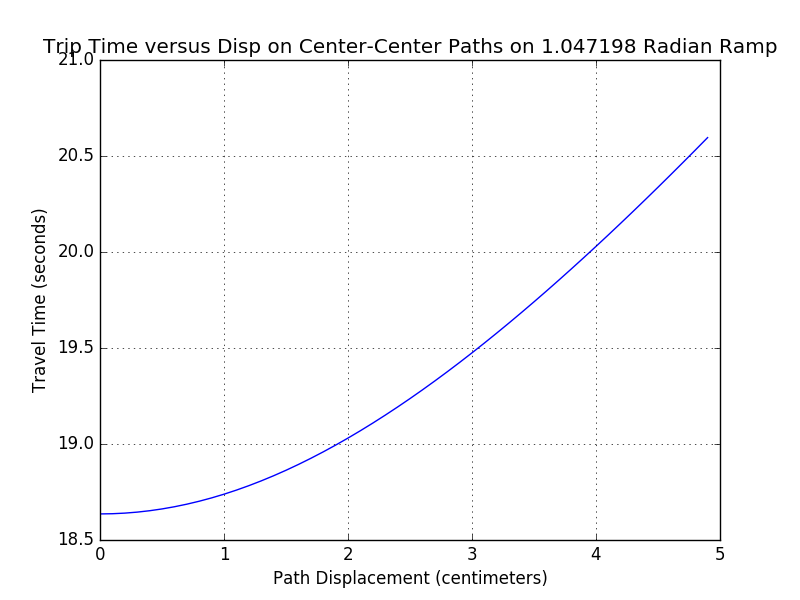
\includegraphics[width=0.2\textwidth]{img/center_center_trip_time_vs_displacement_pi_3_radian_ramp}%
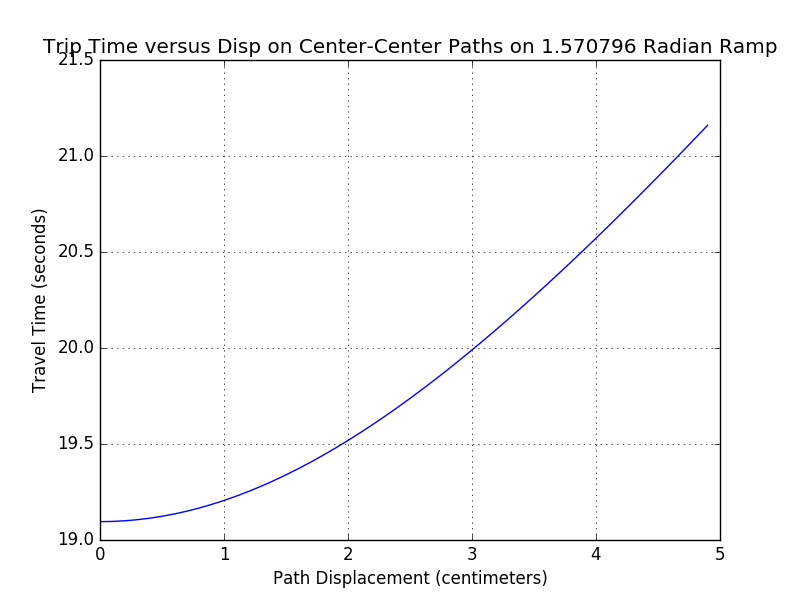
\includegraphics[width=0.2\textwidth]{img/center_center_trip_time_vs_displacement_pi_2_radian_ramp}%
\begin{center}
\begin{tabular}{ c c c }
 incline & displacement (cm) & time (sec) \\ 
 0 & -1.7974794563099371e-07 & 15.405786655568573 \\  
 math.pi/6 & 5.6617903973553256e-07 & 17.122658476770816 \\
 math.pi/4 & 1.0261720572201424e-06 & 18.01885399004196 \\
 math.pi/3 & 5.9487996206179609e-07 & 18.635815540816168 \\
 math.pi/2 & 1.1626086887780648e-06 & 19.09558878811987
\end{tabular} \\
displacement for a direct path: 0
\end{center}


\input{fig/optimalpath_centercenter.tex}

\input{fig/optimalpath_cornercorner.tex}